\documentclass[10pt,fleqn]{article} % Default font size and left-justified equations
\usepackage[%
    pdftitle={Centrale Supelec 2018},
    pdfauthor={UPSTI}]{hyperref}

\input{style/new_style}
\input{style/macros_SII}
\usepackage{multicol}
\usepackage{siunitx}
%\usepackage{picins}
\fichetrue
%\fichefalse

\proftrue
\proffalse

%\tdtrue
\tdfalse

\courstrue
\coursfalse

% -------------------------------------
% Déclaration des titres
% -------------------------------------

\def\discipline{Sciences \\Industrielles de \\ l'Ingénieur}
\def\xxtete{Sciences Industrielles de l'Ingénieur}


\def\classe{\textsf{UPSTI}}
\def\xxnumpartie{CCS 2018}
\def\xxpartie{Modéliser le comportement statique des systèmes mécaniques}

\def\xxnumchapitre{}%Révision 1 \vspace{.2cm}}
\def\xxchapitre{Concours Centrale Supelec PSI 2018}

\def\xxposongletx{2}
\def\xxposonglettext{1.45}
\def\xxposonglety{16}%16

\def\xxonglet{\textsf{Rév -- Stat}}

\def\xxactivite{TD 01}
\def\xxauteur{\textsl{UPSTI}}


\def\xxtitreexo{Tour en fosse utilisé pour le reprofilage des roues ferroviaires}
\def\xxsourceexo{\hspace{.2cm} \footnotesize{Concours Centrale Supelec PSI 2018}}

\def\xxcompetences{%
\textsl{%
%\textbf{Savoirs et compétences :}\\
}}

\def\xxfigures{
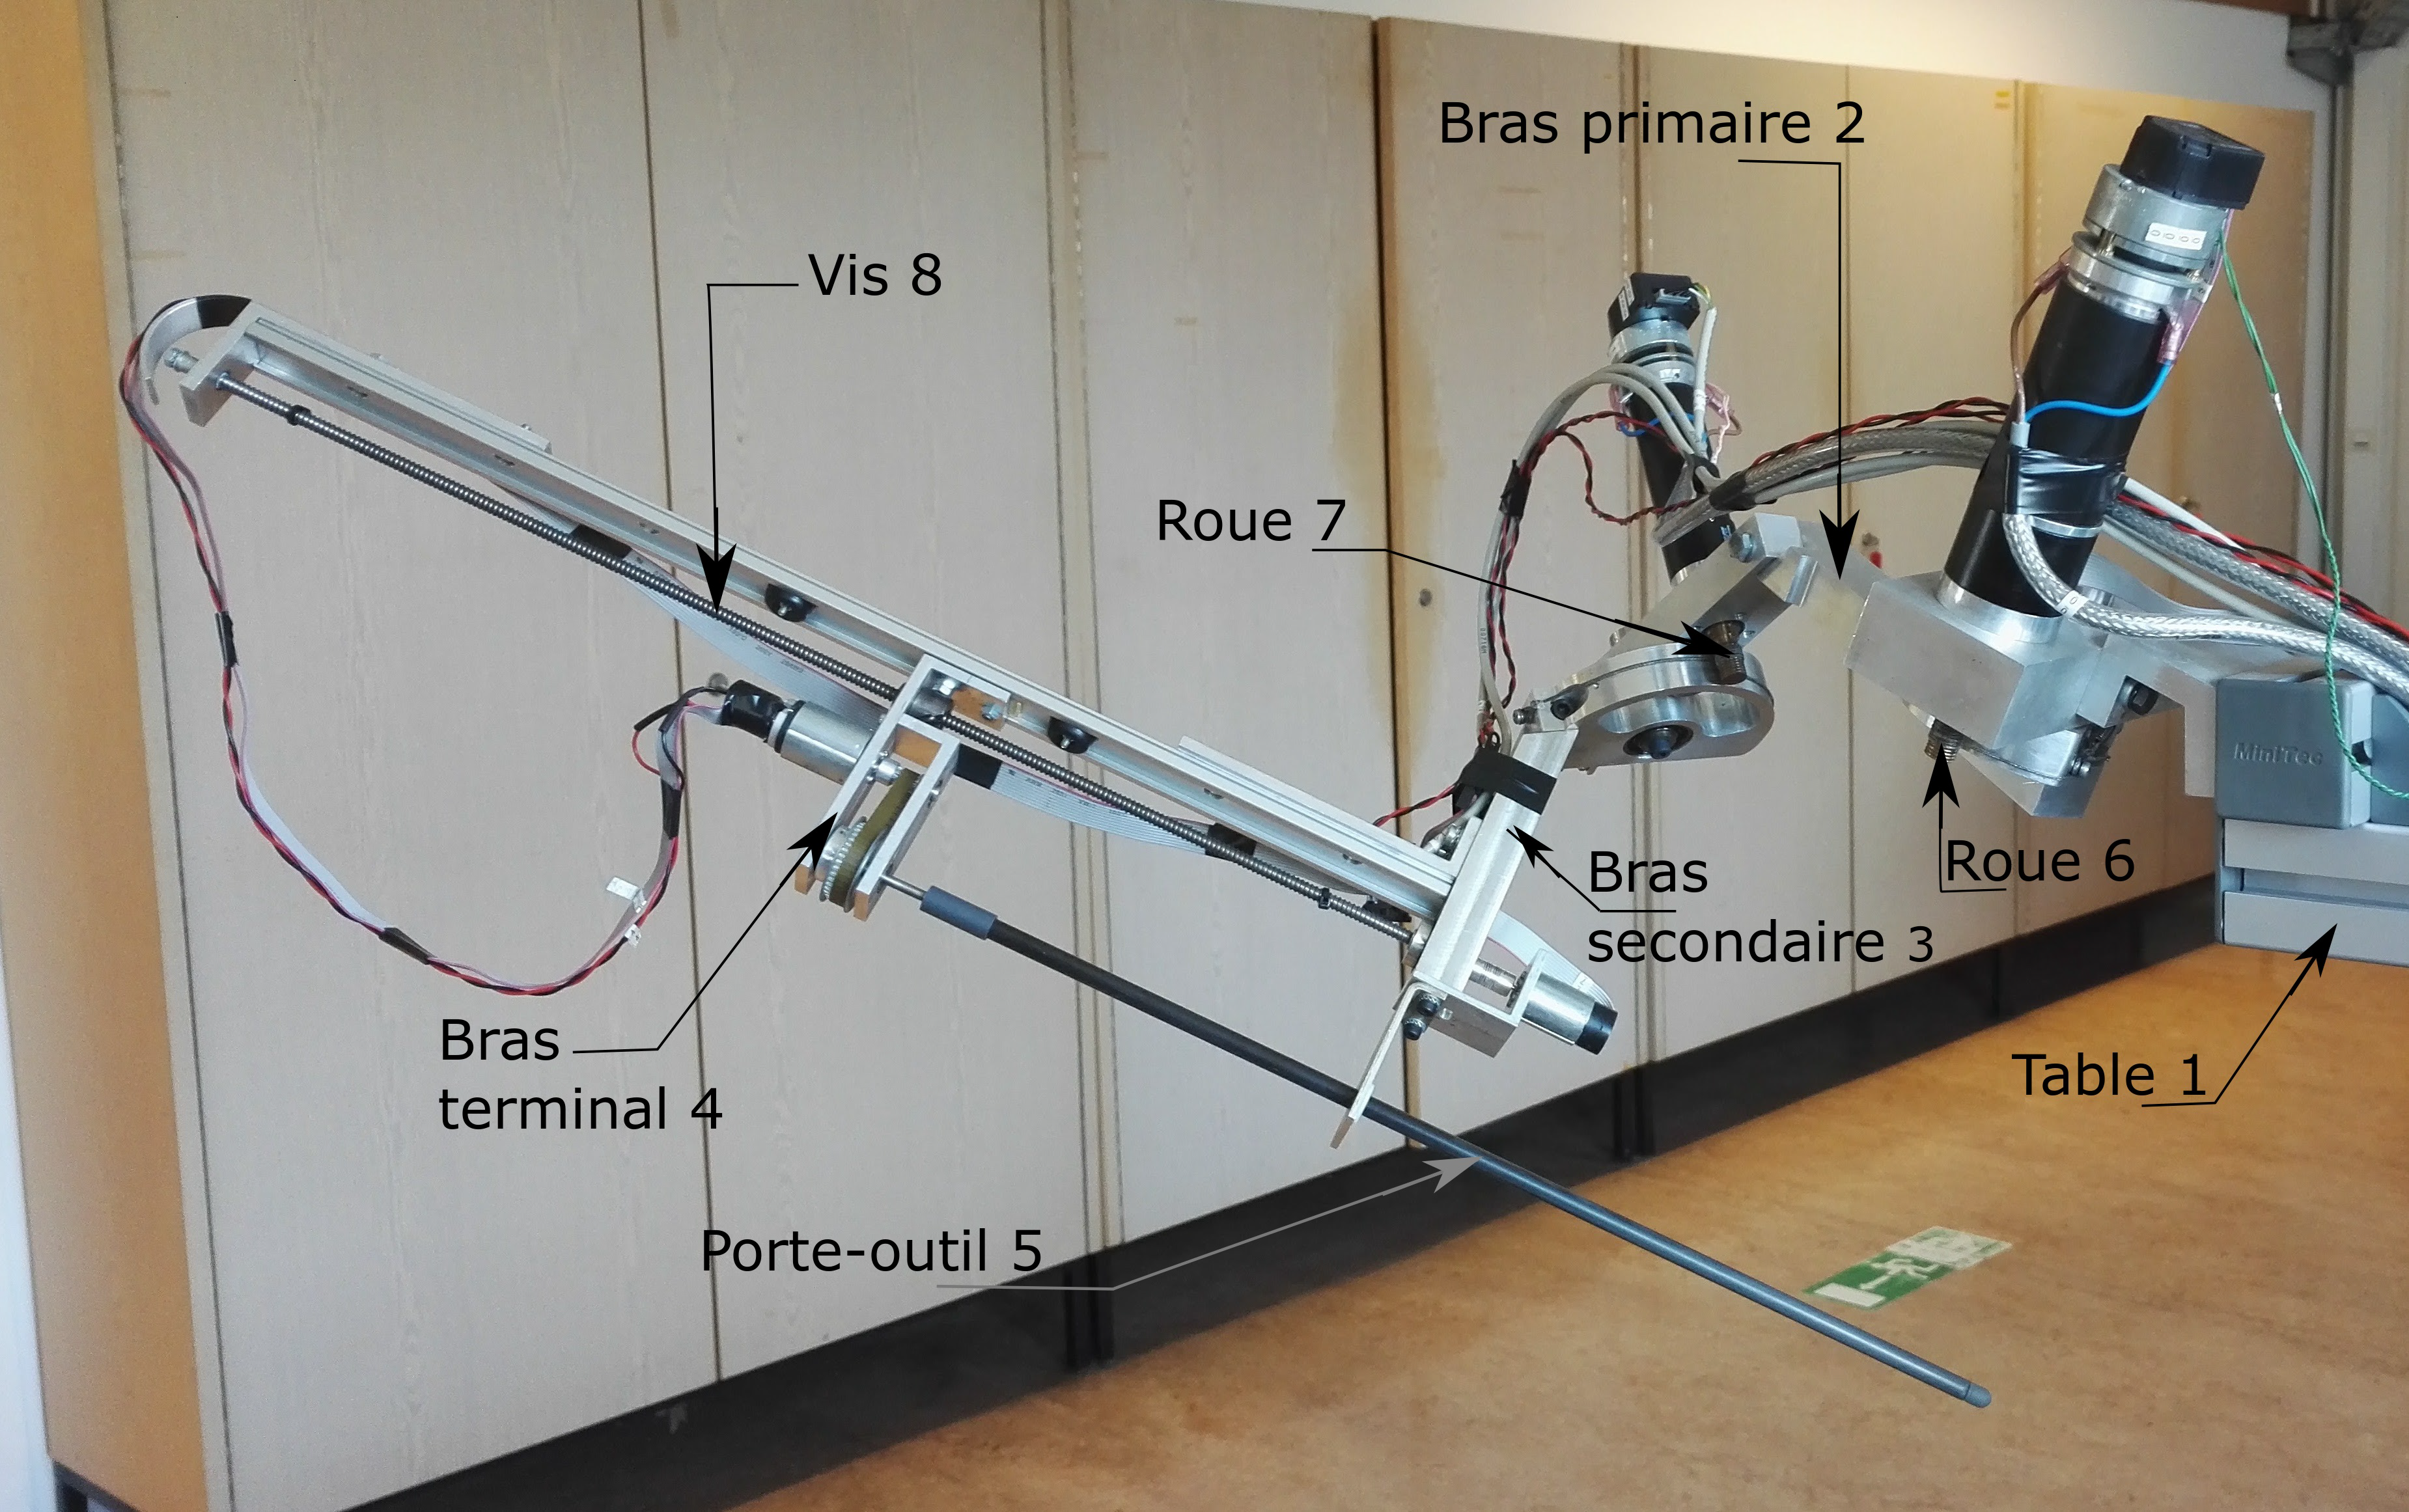
\includegraphics[width=.55\textwidth]{images/fig_00}
}%figues de la page de garde

\def\xxpied{%
Tour en fosse utilisé pour le reprofilage des roues ferroviaires\\
Concours Centrale Supelec -- PSI 2018%
}

\setcounter{secnumdepth}{5}
%---------------------------------------------------------------------------

\usepackage{bm}
\begin{document}
%\chapterimage{png/Fond_Cin}
\input{style/new_pagegarde}
\vspace{4.5cm}
\pagestyle{fancy}
\thispagestyle{plain}


\def\columnseprulecolor{\color{ocre}}
\setlength{\columnseprule}{0.4pt} 

\section{Contexte et étude préliminaire}

\begin{obj}
Valider la pertinence de l’utilisation d’une machine spéciale appelée tour en fosse pour le reprofilage
des roues ferroviaires.
\end{obj}

\subparagraph{}

\begin{itemize}
\item Pour la méthode $a$, $t_{i1} = t_3 +t_4 = \SI{14}{h}= \SI{840}{min}$.
\item Pour la méthode $b$, $t_{i2} = \left( 6\times 3 \times 2 \right)t_5 +t_6 = \SI{545}{min}$.
\end{itemize}

Le gain de temps $\Delta t_i = t_{i1}-t_{i2}=\SI{295}{min}$ soit \SI{4}{h} et \SI{55}{min}. C'est autant de temps gagner sur l'exploitation de la rame. 


.

\section{Analyse de l’entrainement en rotation d’une roue}
\subsection{Description fonctionnelle et structurelle du tour en fosse}
\subsection{Modélisation du dispositif de mise en rotation d’une roue}


\begin{obj}
Vérifier que la modélisation et les hypothèses retenues permettent de déterminer toutes les actions mécaniques nécessaires pour dimensionner les actionneurs des chaines d’énergie.
\end{obj}

\subparagraph{}
À partir des informations données, on peut réaliser le graphe de structure suivant. 

\begin{center}
\includegraphics[width=.7\linewidth]{images/fig_02}
%\textit{}
\end{center}
\begin{multicols}{2}
\textbf{Méthode cinématique}
\begin{itemize}
\item Nombre cyclomatique $\gamma = L-S+1 $ avec $L=5$ liaisons et $S=4$ solides, on a donc $\gamma = 5-4+1=2$ et $E_c=12$ équations cinématiques.
\item Nombre d'inconnues cinématiques : 
\begin{itemize}
\item 3 liaisons pivot : $1\times 3=3$ inconnues;
\item 2 liaisons sphère-plan : $5\times 2=10$ inconnues;
\item \textbf{au total : $I_c=13$ inconnues cinématiques}.
\end{itemize}
\item Mobilités : 
\begin{itemize}
\item mobilités utiles : $m_u=2$ : entrainement des deux moteurs;
\item mobiltés internes : en considérant le glissement entre la roue et les rouleaux, la roue 3, ainsi que $re_1$ et $re_2$ les rouleaux peuvent tourner librement. On a donc : $m_i =3$. %Dans le cas du roulement sans glissement, $m_i=3$;
\item au final, selon les hypothèses, $m=m_i+m_u=5$.
\end{itemize}
\item On a donc $h=m-I_c+E_c =5-13+12=4$.
\end{itemize}

\vfill\null
\columnbreak

\textbf{Méthode statique}
\begin{itemize}
\item 3 solides peuvent être isolés, $E_s=3\times 6 =18$ équations statiques.
\item Nombre d'inconnues statiques : 
\begin{itemize}
\item 3 liaisons pivot : $5\times 3=15$ inconnues;
\item 2 liaisons sphère-plan : $1\times 2=2$ inconnues;
\item \textbf{au total : $I_s=17$ inconnues statiques}.
\end{itemize}
\item Mobilités : $m=m_i+m_u=5$.
\item On a donc $h=m-E_S+I_s =5-18+17=4$.
\end{itemize}
\end{multicols}




%\textbf{Sans tenir compte que les solides 1, 2 et sre sont encastrés au bâti, on est dans les conditions suivantes.}
%
%\begin{center}
%\includegraphics[width=.7\linewidth]{images/fig_01}
%%\textit{}
%\end{center}
%\begin{multicols}{2}
%\textbf{Méthode cinématique}
%\begin{itemize}
%\item Nombre cyclomatique $\gamma = L-S+1 $ avec $L=9$ liaisons et $S=7$ solides, on a donc $\gamma = 9-7+1=3$ et $E_c=18$ équations cinématiques.
%\item Nombre d'inconnues cinématiques : 
%\begin{itemize}
%\item 2 liaisons sphériques : $3\times 2=6$ inconnues;
%\item 4 liaisons pivot : $1\times 4=4$ inconnues;
%\item 1 liaison pivot glissant : 2 inconnues;
%\item 2 liaisons sphère-plan : $5\times 2=10$ inconnues;
%\item \textbf{au total : $I_c=22$ inconnues cinématiques}.
%\end{itemize}
%\item Mobilités : 
%\begin{itemize}
%\item mobilités utiles : $m_u=3$ : entrainement des deux moteurs ainsi que le déploiement du vérin;
%\item mobiltés internes : en considérant le glissement entre la roue et les rouleaux, la roue 3, ainsi que $re_1$ et $re_2$ les rouleaux peuvent tourner librement, rotation propre de la pièce 1 et de la pièce 2 autour du vecteur $\vect{AB}$. On a donc : $m_i =5$. %Dans le cas du roulement sans glissement, $m_i=3$;
%\item au final, selon les hypothèses, $m=m_i+m_u=8$.
%\end{itemize}
%\item On a donc $h=m-I_c+E_c =8-22+18=4$.
%\end{itemize}
%
%\vfill\null
%\columnbreak
%
%\textbf{Méthode statique}
%\begin{itemize}
%\item 6 solides peuvent être isolés, $E_s=6\times 6 =36$ équations statiques.
%\item Nombre d'inconnues statiques : 
%\begin{itemize}
%\item 2 liaisons sphériques : $3\times 2=6$ inconnues;
%\item 4 liaisons pivot : $5\times 4=20$ inconnues;
%\item 1 liaison pivot glissant : 4 inconnues;
%\item 2 liaisons sphère-plan : $1\times 2=2$ inconnues;
%\item \textbf{au total : $I_s=32$ inconnues statiques}.
%\end{itemize}
%\item Mobilités : $m=m_i+m_u=9$.
%\item On a donc $h=m-E_S+I_s =8-36+32=4$.
%\end{itemize}
%\end{multicols}
%
%En utilisant la condition de roulement sans glissement et la méthode cinématique, on ajoute 2 équations cinématiques et $h=3$.

\subparagraph{}
%\begin{multicols}{2}
Condition de roulement sans glissement en $I_1$ : $\vectv{I_1}{3}{re_1} = \vect{0} \Leftrightarrow \vectv{I_1}{3}{0}-\vectv{I_1}{re_1}{0} = \vect{0}$. Par suite, 
\begin{itemize}
\item $\vectv{I_1}{3}{0}=\vectv{O_3}{3}{0}+\vect{I_1 O_3}\wedge \vecto{3}{0} = R\vect{z_1} \wedge \omega_3\vect{y_0}=-R\omega_3 \vect{x_1}$;
\item $\vectv{I_1}{re_1}{0}=\vectv{O_1}{3}{0}+\vect{I_1 O_1}\wedge \vecto{3}{0} = -R_{re}\vect{z_1} \wedge \omega_{re_1}\vect{y_0}=R_{re}\omega_{re_1} \vect{x_1}$.
\end{itemize}
On a donc $-R\omega_3 -R_{re}\omega_{re_1} =0 \Leftrightarrow\dfrac{\omega_3}{\omega_{re_1}}=-\dfrac{R_{re}}{R} $.
%\end{multicols}

De même en exploitant le roulement sans glissement en $I_2$, $\dfrac{\omega_3}{\omega_{re_2}}=-\dfrac{R_{re}}{R} $. 

La condition de roulement sans glissement supprime les 3 mobilités internes; donc $m'=2$ et $h'=1$. 

\subparagraph{}
Dans les conditions précédentes, les couples $\mathcal{C}_{mi}$ ne peuvent pas être déterminés. Il faudrait imposer un taux de rotation rigoureusement identique pour $\omega_{re_1}$ et $\omega_{re_2}$. 


\subsection{Motorisation du dispositif de mise en rotation d'une roue}
\begin{obj}
Analyser la chaine d’entrainement en rotation d’une roue et vérifier le choix de la machine électrique.
\end{obj}

\subparagraph{}
On conserve l'hypothèse que $sre$ est supposé fixe par rapport au bâti. 
On a $E_1=M_1+R_1+re_1$. Ces 3 solides sont en liaison pivot par rappor tau bâti. En conséquence, 
$T\left(E_1/0\right)=T\left(M_1/0\right)+T\left(R_1/0\right)+T\left(re_1/0\right) = \dfrac{1}{2}J_m\omega_m^2+\dfrac{1}{2}J_{re}\omega_{re}^2+\dfrac{1}{2}J_{re}\omega_{re}^2=\dfrac{1}{2}\left(J_m+J_{red}k^2+J_{re}k^2\left( \dfrac{R_{re}}{R}\right)^2 \right) \omega_m^2$.

On a donc $J_{eq}=J_m+J_{red}k^2+J_{re}k^2\left( \dfrac{R_{re}}{R}\right)^2$.

\subparagraph{}
On prend le graphe de structure suivant :
\begin{center}
\includegraphics[width=.5\linewidth]{images/fig_03}
%\textit{}
\end{center}

On isole $E_1$. Bilan des puissances internes : les liaisons internes au système considrée sont considérées sans frottement. On a donc : $\mathcal{P}_{\text{int}}\left(E_1\right)=0$.

Bilan des puissances externes : 
\begin{itemize}
\item la puissance développée par le moteur peut s'exprimer par $\mathcal{P}\left(\text{sre}\to M_1/0\right)=C_m\omega_m$;
\item puissance développée par l'action de 3 sur $\text{re}_1$ : $\mathcal{P}\left(3\to \text{re}_1/0\right)=\torseurcin{V}{\text{re}_1}{0}\otimes\torseurstat{T}{3}{\text{re}_1}=\torseurl{k\omega_m \vect{y_0}}{kR_{re}\omega_m\vect{x_1}}{I_1}\otimes
\torseurl{-F_{z1}\vect{z_1}-F_{x1}\vect{x_1}}{\vect{0}}{I_1}= -kR_{re}F_{x1}\omega_m$.
\end{itemize}

On applique le théorème de l'énergie cinétique et $\dfrac{\dd T\left(E_1/0\right)}{\dd t}= C_m\omega_m-kR_{re}F_{x1}\omega_m \Rightarrow \dot{\omega}_m J_{eq}= C_m-kR_{re}F_{x1} $.

\subparagraph{}
En isolant l'ensemble $E_2=\left\{M_2+R_2+re_2\right\}$ et en appliquant le théorème de l'énergie cinétique : $\dot{\omega}_m J_{eq}= C_m-kR_{re}F_{x2}$. Comme les caractéristiques des deux chaînes d'entrainement sont les mêmes, on a donc nécessairement $F_{x1}=F_{x2}$.

\subparagraph{}
On a vu que $\dfrac{\omega_3}{\omega_{re_1}}=-\dfrac{R_{re}}{R}$ de plus $\omega_{re_1}=k\omega_m$; donc $\omega_3= -k\dfrac{R_{re}}{R}\omega_m$. En dérivant, on a $\dot{\omega_3}= -k\dfrac{R_{re}}{R}\dot{\omega}_m$.


\subparagraph{}
\textbf{Stratégie :} on cherche à exrimer le couple moteur en fonction des grandeurs du géométriques, inertielles, ... pour cela, la roue étant en pivot d'axe $\axe{O}{y_0}$ on va réaliser un théorème du moment dynamique en $O_3$ en projection sur $\vect{y_0}$. 

On isole la roue \textbf{3}.

On réalise le bilan des actions mécaniques extérieures : 
\begin{itemize}
\item action de la pivot en $O_3$;
\item action des liaisons sphères plans : 
\begin{itemize}
\item $\vectm{O_3}{re_1}{3}\cdot \vect{y_0} = \left(\vect{O_3 I_1} \wedge \left(  F_{x1}\vect{x_1}+F_{z1}\vect{z_1}\right) \right) \cdot \vect{y_0}
= \left(-R\vect{z_1} \wedge \left(  F_{x1}\vect{x_1}+F_{z1}\vect{z_1}\right) \right) \cdot \vect{y_0}
= -RF_{x1}$.
\item $\vectm{O_3}{re_2}{3}\cdot \vect{y_0} 
= \left(\vect{O_3 I_2} \wedge \left(  F_{x2}\vect{x_2}+F_{z2}\vect{z_2}\right) \right) \cdot \vect{y_0}
= \left(-R\vect{z_2} \wedge \left(  F_{x2}\vect{x_2}+F_{z2}\vect{z_2}\right) \right) \cdot \vect{y_0}
= -RF_{x2}$.
\end{itemize}
\item action de l'outil :
$\vectm{O_3}{\text{outil}}{3}\cdot \vect{y_0} 
= \left(\vect{O_3 C} \wedge \vectf{\text{outil}}{3} \right) \cdot \vect{y_0}
= \left( \vectf{\text{outil}}{3} \wedge \vect{y_0}\right) \cdot \vect{O_3 C}
= \left( \vectf{\text{outil}}{3} \wedge \vect{y_0}\right) \cdot \vect{O_3 C}
$.
\end{itemize}
En faisant l'hypothèse que le moteur tourne dans le sens direct, la roue tourne dans le sens horaire. On peut alors déduire les signes des efforts normaux et tangentiels. Ainis, $F_{x1}=-f F_{z1}$. 
\begin{center}
\includegraphics[width=.5\linewidth]{images/fig_04}
%\textit{}
\end{center}

 
Ainsi :
\begin{itemize}
\item $\torseurstat{T}{re_1}{3} = \torseurl{F_{z1}\vect{z_1}+F_{x1}\vect{x_1}}{\vect{0}}{I_1}$. 
\end{itemize}
\end{document}

\subparagraph{}\textit{}


\begin{center}
\includegraphics[width=\linewidth]{images/img_04}
%\textit{}
\end{center}

